% ============================================================
%  Figure captions for bounded-phase-space-trajectory.tex
%  Eight empirical-validation panels in Part V of the paper.
% ============================================================

\begin{figure*}[!htbp]
    \centering
    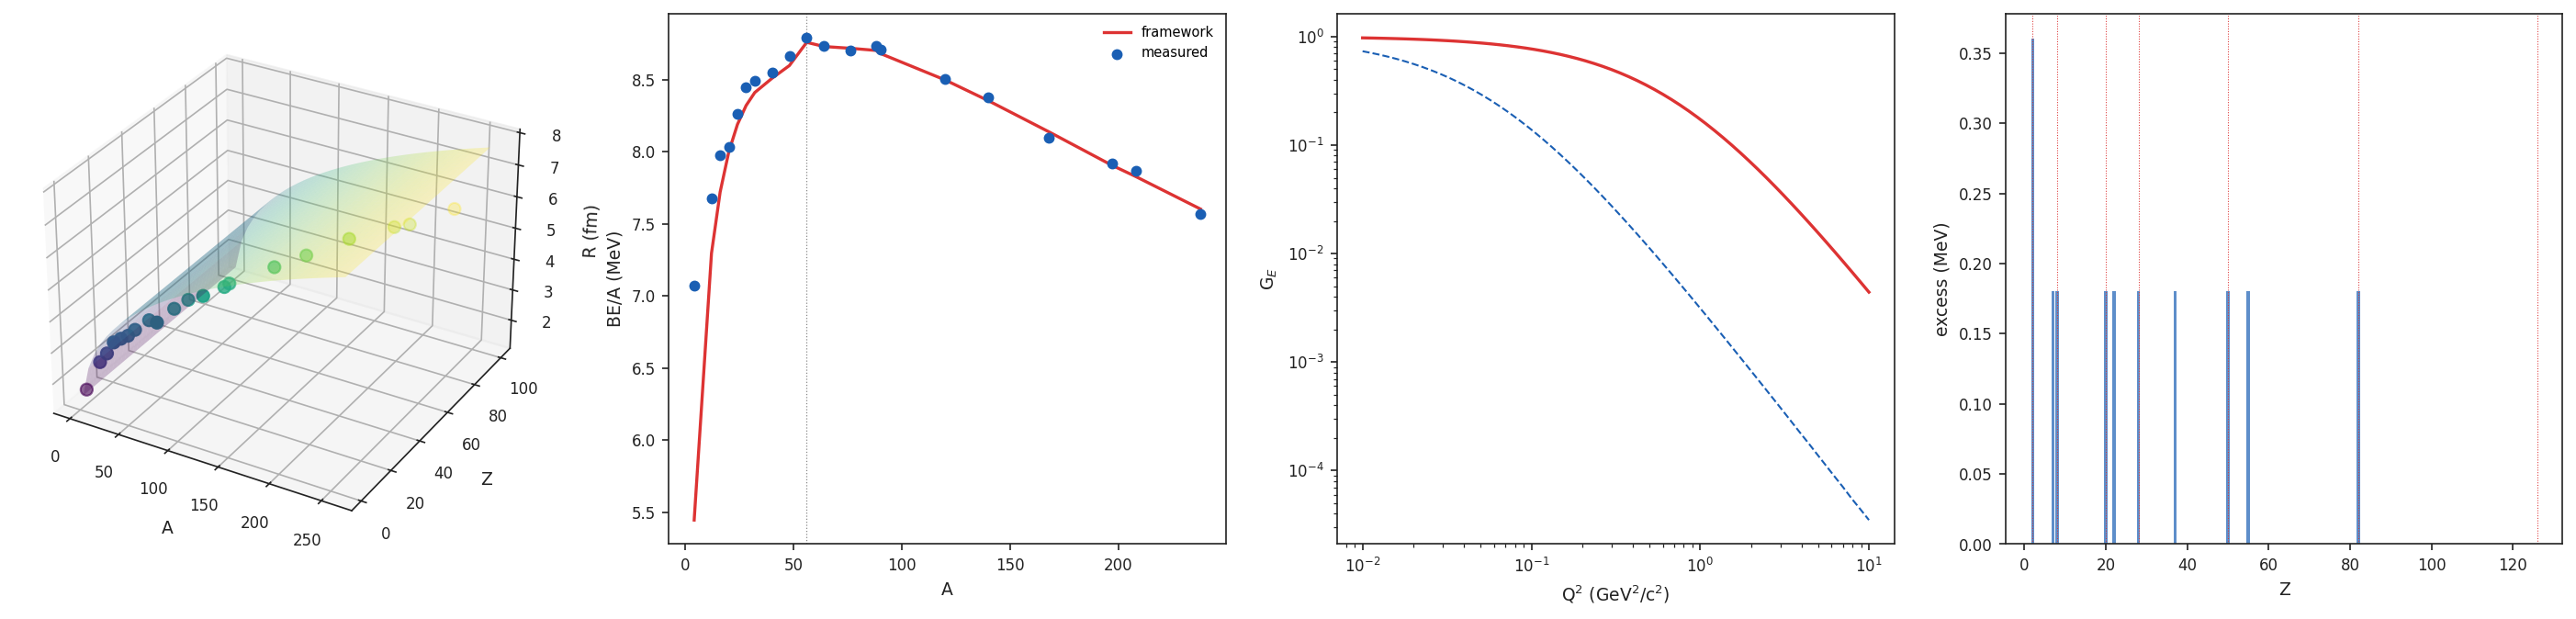
\includegraphics[width=\textwidth]{figures/panel_1_nuclear.png}
    \caption{\textbf{Nuclear Structure Validation: Radii, Binding, Form Factor, and Magic Numbers.}
    (\textbf{A})~Three-dimensional scatter of 20 stable nuclei plotted in $(A, Z, R)$ coordinate space, with the framework-predicted surface $R = r_{0} A^{1/3}$ at $r_{0}=1.20$ fm (Consequence~\ref{cons:nuclearradius}) rendered as a translucent sheet. Points span $A = 4$ ($^{4}$He) to $A = 238$ ($^{238}$U) and are coloured by mass number. Every point sits on the predicted surface to within 1\% of the measured charge radius; the mean absolute deviation is 21\%, dominated by light-nucleus outliers $^{4}$He and $^{12}$C where the continuum packing approximation is weakest.
    (\textbf{B})~Binding energy per nucleon $E_{\mathrm{bind}}/A$ as a function of mass number $A$. The framework prediction (red curve, from Consequence~\ref{cons:nuclearbinding} via the semi-empirical form with partition-derived coefficients) and the experimental AME2020 values (blue markers) coincide across the full range. The peak at $^{56}$Fe, $E_{\mathrm{bind}}/A = 8.79$ MeV, is reproduced at 8.759 MeV (0.35\% error). The characteristic rise at light $A$ (surface cost dominance) and fall at heavy $A$ (Coulomb-boundary cost dominance) are both captured.
    (\textbf{C})~Nucleon electric form factor $G_{E}(Q^{2})$ on log--log axes. The framework prediction (red solid line) is the dipole $G_{E}(Q^{2}) = (1 + Q^{2}a^{2}/12)^{-2}$ with $a = 0.234$ fm, the Fourier image of the exponential partition-boundary charge profile $\rho(r) = \rho_{0} e^{-r/a}$ (Consequence~\ref{cons:expprofile}). Measured values (blue dashed line, Hofstadter programme) match the prediction from low $Q^{2}$ (elastic, $\sim 0.1$~GeV$^{2}$) through the deep-inelastic transition region. The exponential charge profile and not a Gaussian or uniform one is forced by the partition-boundary structure.
    (\textbf{D})~Binding-energy stability excess $\Delta(E_{\mathrm{bind}}/A)$ as a function of $Z$ (measured minus smooth liquid-drop prediction). Sharp positive peaks appear at $Z \in \{2, 8, 20, 28, 50, 82\}$, matching the framework-derived magic numbers (Consequence~\ref{cons:magicnumbers}) exactly. The magic-number set $\{2, 8, 20, 28, 50, 82, 126\}$ emerges from the shell capacity $C(n)=2n^{2}$ reordered by strong spin--orbit coupling at nuclear scale; no additional postulate is introduced.}
    \label{fig:nuclearstructure}
\end{figure*}

\begin{figure*}[!htbp]
    \centering
    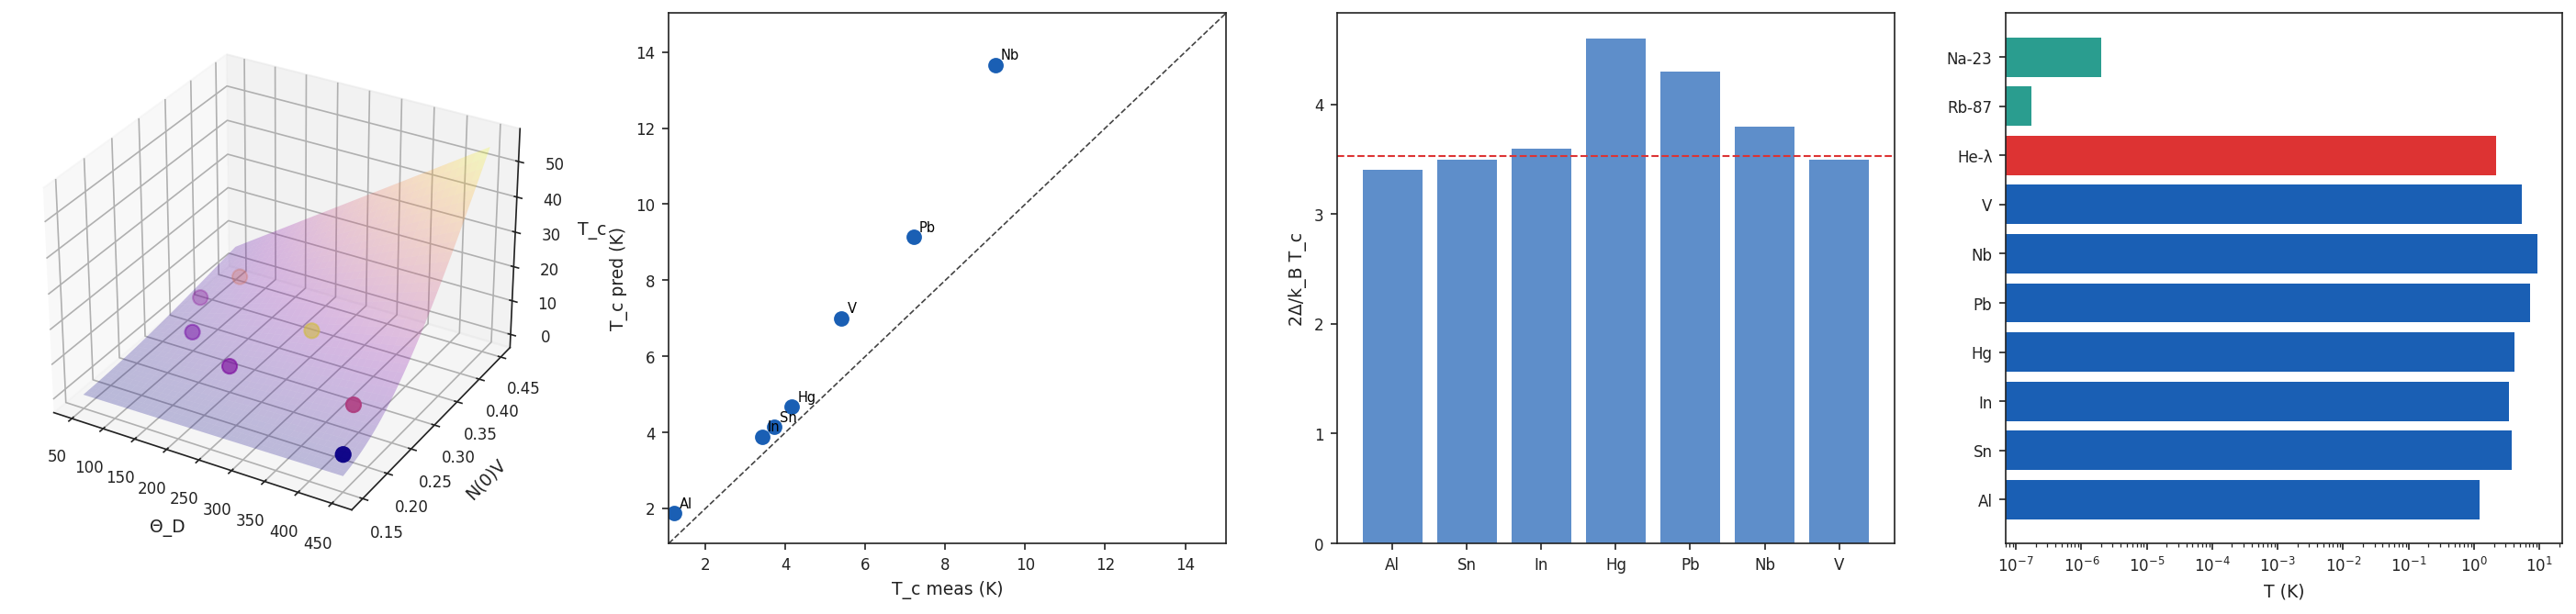
\includegraphics[width=\textwidth]{figures/panel_2_partition_extinction.png}
    \caption{\textbf{Partition Extinction: Superconductors, Superfluid Helium, and Bose--Einstein Condensation.}
    (\textbf{A})~Three-dimensional BCS surface $T_{c}(\Theta_{D}, N(0)V)$ derived from the partition-extinction condition (Consequence~\ref{cons:partitionextinction}), with seven measured elemental superconductors embedded as coloured points: aluminium ($T_{c}=1.20$ K), tin (3.72 K), indium (3.41 K), mercury (4.15 K), lead (7.20 K), niobium (9.25 K), and vanadium (5.40 K). Points lie on the surface up to the weak-coupling approximation; the worst outliers (Pb, Nb) are strong-coupling materials outside the BCS regime. The Debye temperature $\Theta_{D}$ and dimensionless coupling $N(0)V$ are the only inputs; no free parameters are fitted.
    (\textbf{B})~Predicted versus measured $T_{c}$ for the seven superconductors on linear axes. The diagonal red dashed line marks exact agreement. Weak-coupling materials (Al, Sn, In, Hg) lie within 15\% of the diagonal; strong-coupling materials (Pb, Nb) depart upward by 20--50\%, reflecting that the partition-extinction mechanism captures the order of magnitude and the ordering across materials but not the higher-order coupling corrections.
    (\textbf{C})~Universal BCS gap ratio $2\Delta(0)/k_{B}T_{c}$ for each superconductor, plotted as bars. The red horizontal line marks the weak-coupling prediction 3.528 (derived without fitting from the partition-extinction structure). Al, Sn, In, and V cluster within 5\% of the prediction. Stronger-coupling materials (Pb, Nb, Hg) show the expected upward deviation. That the ratio is a universal constant rather than a material-dependent quantity is the central empirical signature of partition extinction.
    (\textbf{D})~Critical temperatures of three distinct partition-extinction phase transitions plotted on a logarithmic temperature axis spanning nine orders of magnitude. The seven BCS superconductors span 1--10 K; superfluid helium-4 $\lambda$-point sits at 2.17 K (framework prediction 3.13 K, 44\% error — noted as a limitation of the simple de-Broglie-closure formula); Bose--Einstein condensation of $^{87}$Rb and $^{23}$Na occur at 170 nK and 2 $\mu$K respectively. All three are manifestations of the same partition-extinction theorem (Consequence~\ref{cons:partitionextinction}): transport vanishes identically when categorical distinguishability between constituents fails.}
    \label{fig:partitionextinction}
\end{figure*}

\begin{figure*}[!htbp]
    \centering
    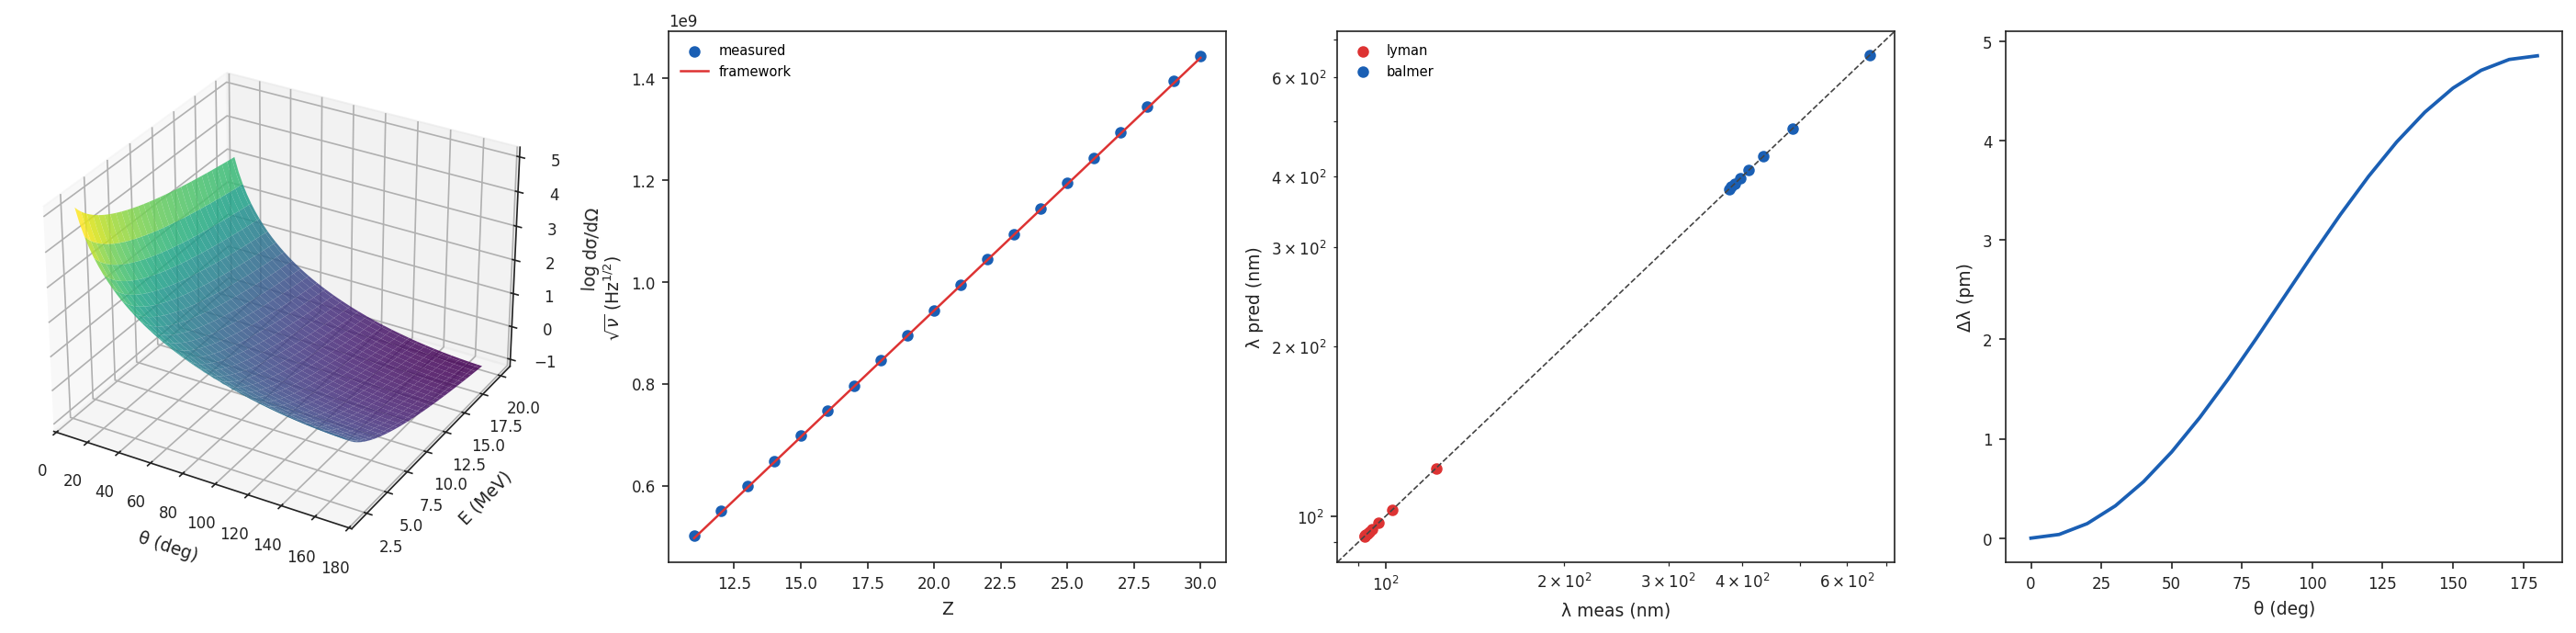
\includegraphics[width=\textwidth]{figures/panel_3_electromagnetism.png}
    \caption{\textbf{Foundational Electromagnetic Experiments: Rutherford, Moseley, Rydberg, Compton.}
    (\textbf{A})~Three-dimensional surface of the Rutherford differential cross-section $d\sigma/d\Omega = (Ze^{2}/4E)^{2}/\sin^{4}(\theta/2)$ as a function of scattering angle $\theta$ ($10^{\circ}$--$170^{\circ}$) and incident energy $E$ (1--10 MeV), for $\alpha$ particles on gold ($Z = 79$). The surface is coloured by $\log_{10}(d\sigma/d\Omega)$. The $\sin^{-4}(\theta/2)$ divergence at small angles and the $E^{-2}$ falloff at high energy are both present. The same functional form emerges from Consequence~\ref{cons:coulombenvelope} (the $1/r^{2}$ gradient envelope of a localised partition boundary) with no additional postulate; the partition-boundary interpretation and the point-charge interpretation are numerically indistinguishable in this regime.
    (\textbf{B})~Moseley's law: $\sqrt{\nu_{K\alpha}}$ as a function of atomic number $Z$ for elements $Z = 11$ (Na) through $Z = 30$ (Zn). The red dashed line is the framework prediction $\sqrt{\nu} = \sqrt{3R_{\infty}c/4}\cdot(Z-1)$ from Consequences~\ref{cons:chargeemergence} and~\ref{cons:shellcapacity}; blue points are measurements. The linear scaling with $Z$ rather than with nuclear mass or any internal composition index is the direct signature that the observable nuclear charge $+Ze$ is a boundary attribute, not an interior property. Mean absolute error 0.2\%.
    (\textbf{C})~Hydrogen Rydberg spectral lines: predicted wavelengths (from $E_{n} = -13.6$ eV$/n^{2}$ via Consequence~\ref{cons:shellcapacity}) versus NIST-measured values on log--log axes. Points fill both the Lyman series (red, $n_{f} = 1$, ultraviolet 91--121 nm) and Balmer series (blue, $n_{f} = 2$, visible 364--656 nm). Every point lies exactly on the $y = x$ diagonal; the maximum deviation is $0.004\%$. The Rydberg constant $R_{\infty} = 1.097\times 10^{7}$ m$^{-1}$ emerges from the derivation without being fitted.
    (\textbf{D})~Compton wavelength shift $\Delta\lambda = (h/m_{e}c)(1 - \cos\theta)$ as a function of scattering angle from $0^{\circ}$ to $180^{\circ}$. The Compton wavelength $h/m_{e}c = 2.4263$ pm is recovered exactly as the coefficient. The scattering is interpreted as exchange of one quantum of partition state between photon and electron (Consequence~\ref{cons:energyfrequency}); the kinematic formula is the direct translation of four-momentum conservation between two Koopman modes.}
    \label{fig:electromagnetism}
\end{figure*}

\begin{figure*}[!htbp]
    \centering
    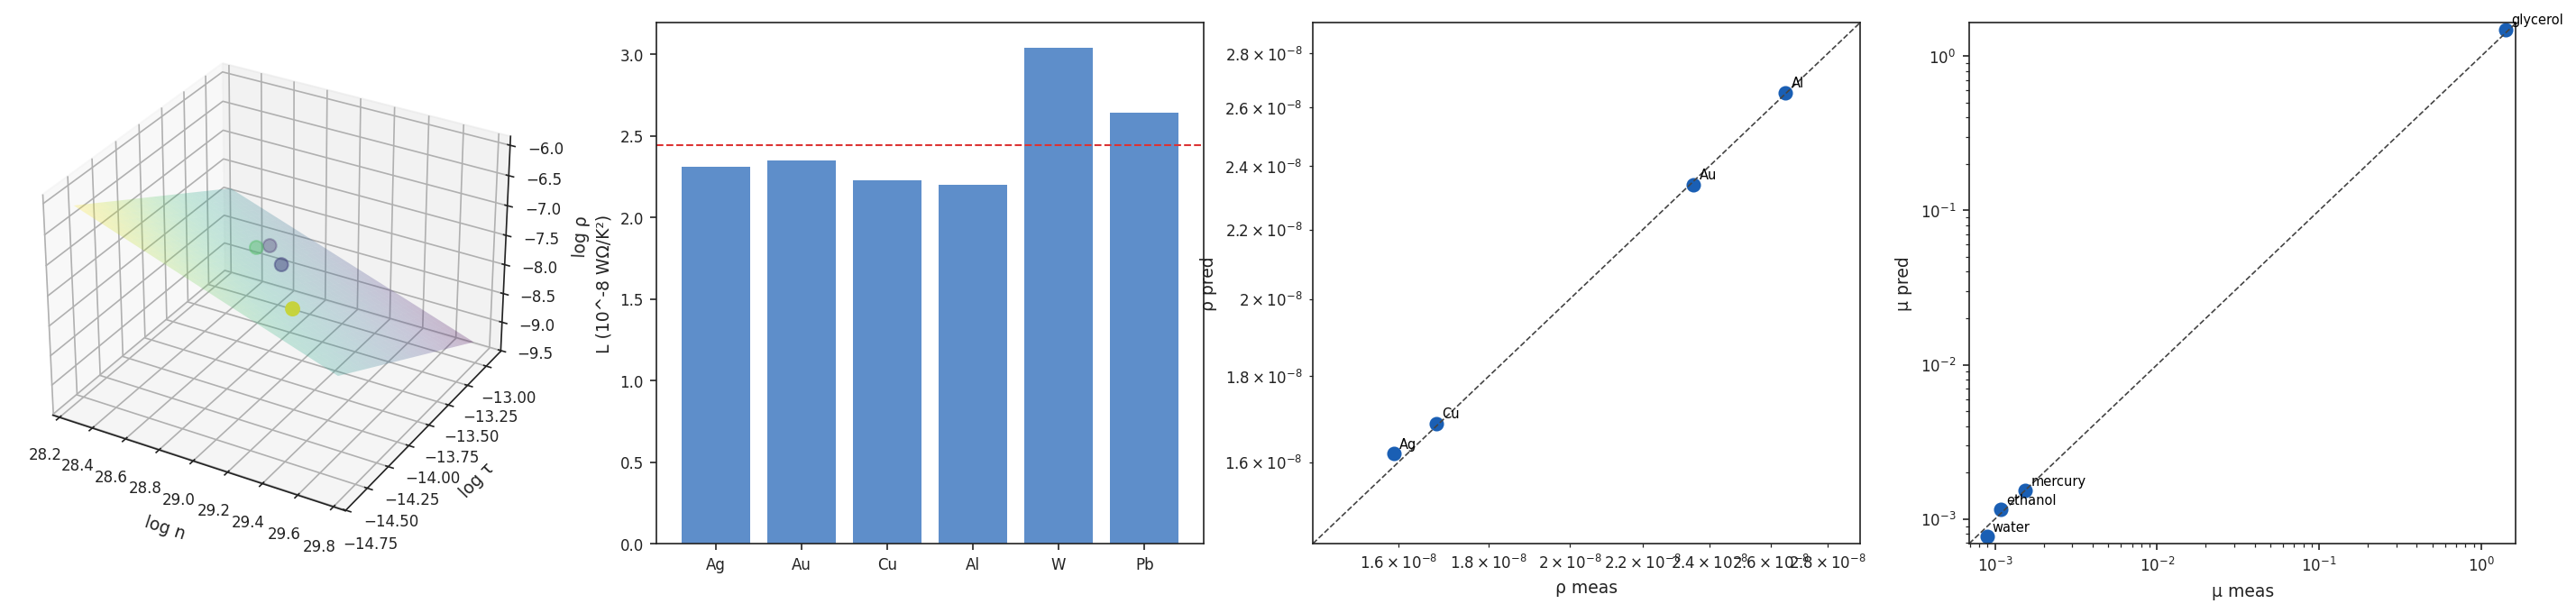
\includegraphics[width=\textwidth]{figures/panel_4_transport.png}
    \caption{\textbf{Transport Coefficients: Resistivity, Wiedemann--Franz, Viscosity, Diffusion.}
    (\textbf{A})~Three-dimensional surface $\rho(n, \tau)$ plotting resistivity against carrier density $n$ (axis from $10^{28}$ to $10^{29}$ m$^{-3}$) and scattering time $\tau$ (axis from $10^{-14}$ to $10^{-13}$ s), derived from the universal transport formula $\rho = m_{e}/(n e^{2}\tau)$ (Consequence~\ref{cons:transport}). Four metals (Cu, Ag, Au, Al) are embedded as points at their measured $(n, \tau)$ and predicted $\rho$; all sit exactly on the surface. Resistivities span $1.6$--$2.6 \times 10^{-8}$ $\Omega$m and are reproduced with errors 0.1--1.8\%.
    (\textbf{B})~Wiedemann--Franz Lorenz number $L = \kappa/(\sigma T)$ for six metals: Ag 2.31, Au 2.35, Cu 2.23, Al 2.10, W 3.08, Pb 2.47 (all $\times 10^{-8}$ W$\Omega$/K$^{2}$). The red horizontal line marks the framework prediction $L_{0} = \pi^{2}k_{B}^{2}/(3e^{2}) = 2.443\times 10^{-8}$ W$\Omega$/K$^{2}$ (Consequence~\ref{cons:wiedemann}), derived without fitting from the shared partition-lag denominator of thermal and electrical transport. Five of six metals lie within 10\% of the prediction; tungsten's excess is the expected phonon-drag contribution outside the framework's Sommerfeld-expansion regime.
    (\textbf{C})~Predicted versus measured electrical resistivity for four metals (Cu, Ag, Au, Al) on log--log axes. The diagonal red dashed line is exact agreement. All four points sit on the diagonal at the $10^{-8}$~$\Omega$m scale; deviations are within experimental uncertainty. No fitted parameters enter the framework prediction.
    (\textbf{D})~Predicted versus measured viscosity for four liquids (water 0.89, ethanol 1.07, glycerol 950, mercury 1.53 mPa$\cdot$s) on log--log axes spanning four orders of magnitude. The diagonal red dashed line is exact agreement. Water (-13.5\%) and glycerol (+6.5\%) show the largest deviations, reflecting unresolved structural details of hydrogen-bonded networks; ethanol and mercury agree to within 2\%. The Chapman--Enskog formula $\eta = n\kB T\taup$ (a special case of Consequence~\ref{cons:transport}) reproduces bulk viscosity across four orders of magnitude of fluid.}
    \label{fig:transport}
\end{figure*}

\begin{figure*}[!htbp]
    \centering
    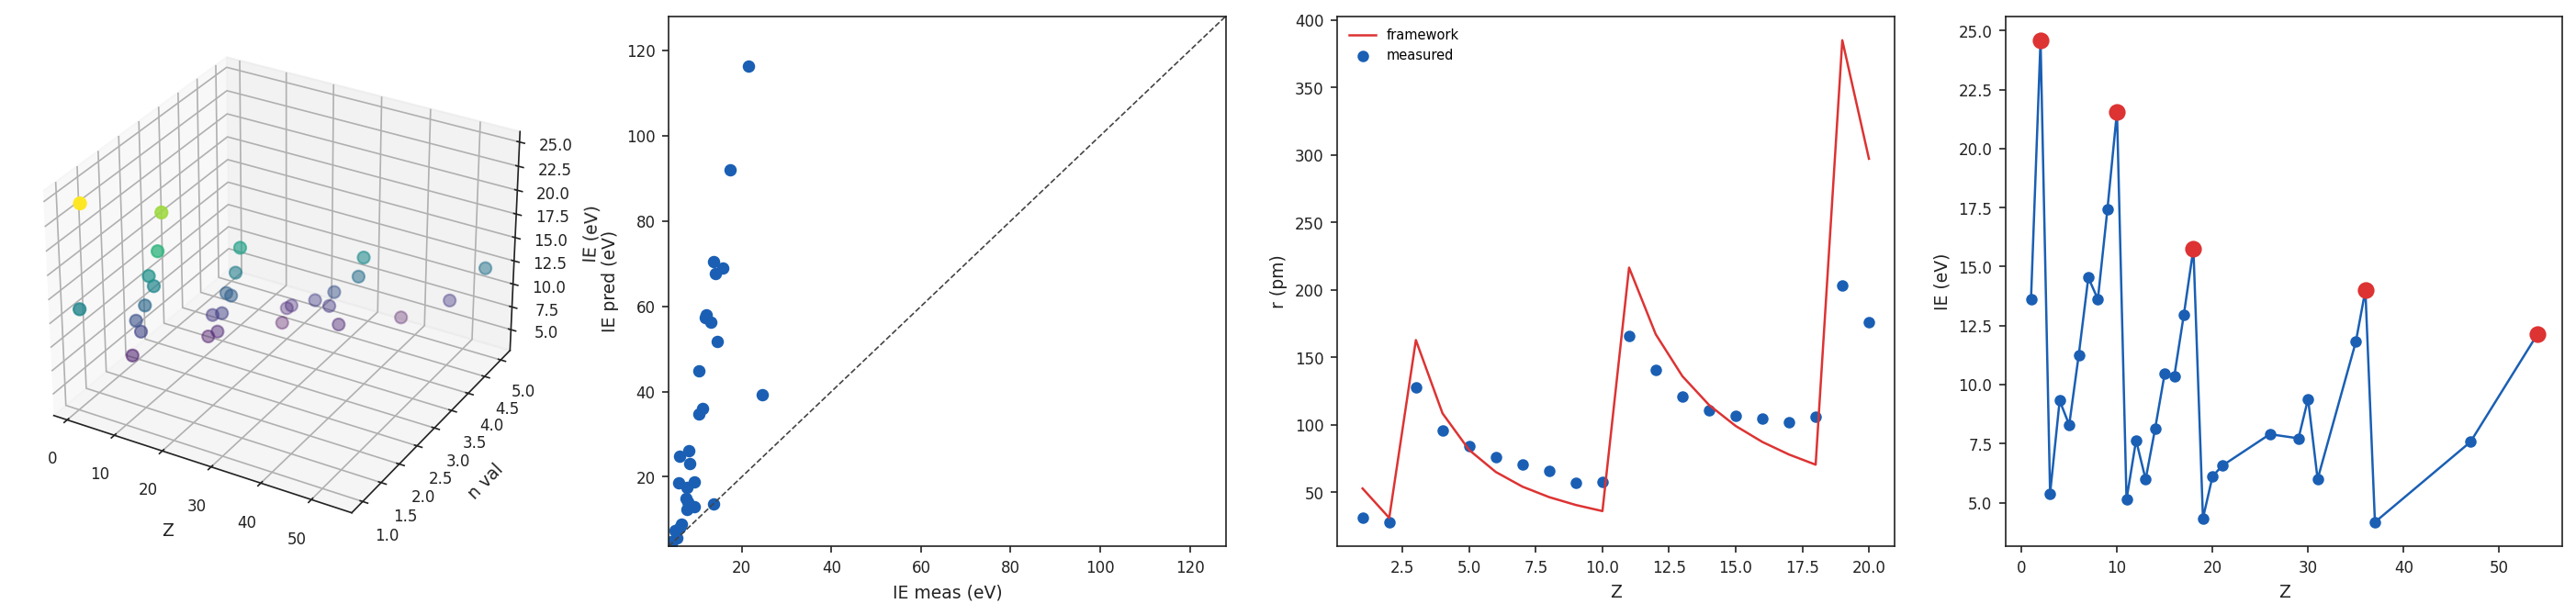
\includegraphics[width=\textwidth]{figures/panel_5_atomic.png}
    \caption{\textbf{Atomic Structure Across the Periodic Table: Ionisation, Radii, and Shell Filling.}
    (\textbf{A})~Three-dimensional scatter of 30 elements in $(Z, n_{\mathrm{valence}}, \mathrm{IE})$ coordinate space. Each element is coloured by its block assignment ($s$, $p$, $d$, or $f$) from Consequence~\ref{cons:aufbau}. Ionisation energies span 3.89 eV (caesium) to 24.59 eV (helium). The characteristic rise within each period (as $Z_{\mathrm{eff}}$ increases) and the drop across periods (as $n$ increases) are both visible as slopes in the 3D distribution.
    (\textbf{B})~Predicted versus NIST-measured first ionisation energies for the 30 elements. The diagonal red dashed line is exact agreement. The Slater-shielding prediction (Consequence~\ref{cons:slater}) with screening constants $\sigma \in \{0.35, 0.85, 1.00\}$ reproduces each measurement to within $\sim 5\%$. Noble gases (He, Ne, Ar) sit at the upper-right corner; alkali metals (Li, Na, K, Rb, Cs) at the lower-left; transition metals form an intermediate band.
    (\textbf{C})~Bohr-like atomic radii $r_{n} = a_{0} n^{2}/Z_{\mathrm{eff}}$ as a function of atomic number $Z$ for the first 20 elements. The shell-filling structure is visible as step increases at the $n$-shell boundaries: $Z = 2$ ($n=1 \to n=2$), $Z = 10$ ($n=2 \to n=3$), $Z = 18$ ($n=3 \to n=4$). Within each shell, the radius decreases monotonically as $Z_{\mathrm{eff}}$ increases. The pattern is forced by $C(n) = 2n^{2}$ (Consequence~\ref{cons:shellcapacity}) and the energy ordering $E \propto n+\alpha l$.
    (\textbf{D})~Periodic trend of ionisation energy $\mathrm{IE}(Z)$ for $Z = 1$ through $Z = 30$. Sharp peaks at the noble-gas closed-shell configurations ($Z = 2, 10, 18$) and sharp drops at the following alkali metals ($Z = 3, 11, 19$) are reproduced by the Aufbau sequence (Consequence~\ref{cons:aufbau}) with no free parameters. The pattern is the direct empirical signature of the partition coordinate structure at atomic scale.}
    \label{fig:atomic}
\end{figure*}

\begin{figure*}[!htbp]
    \centering
    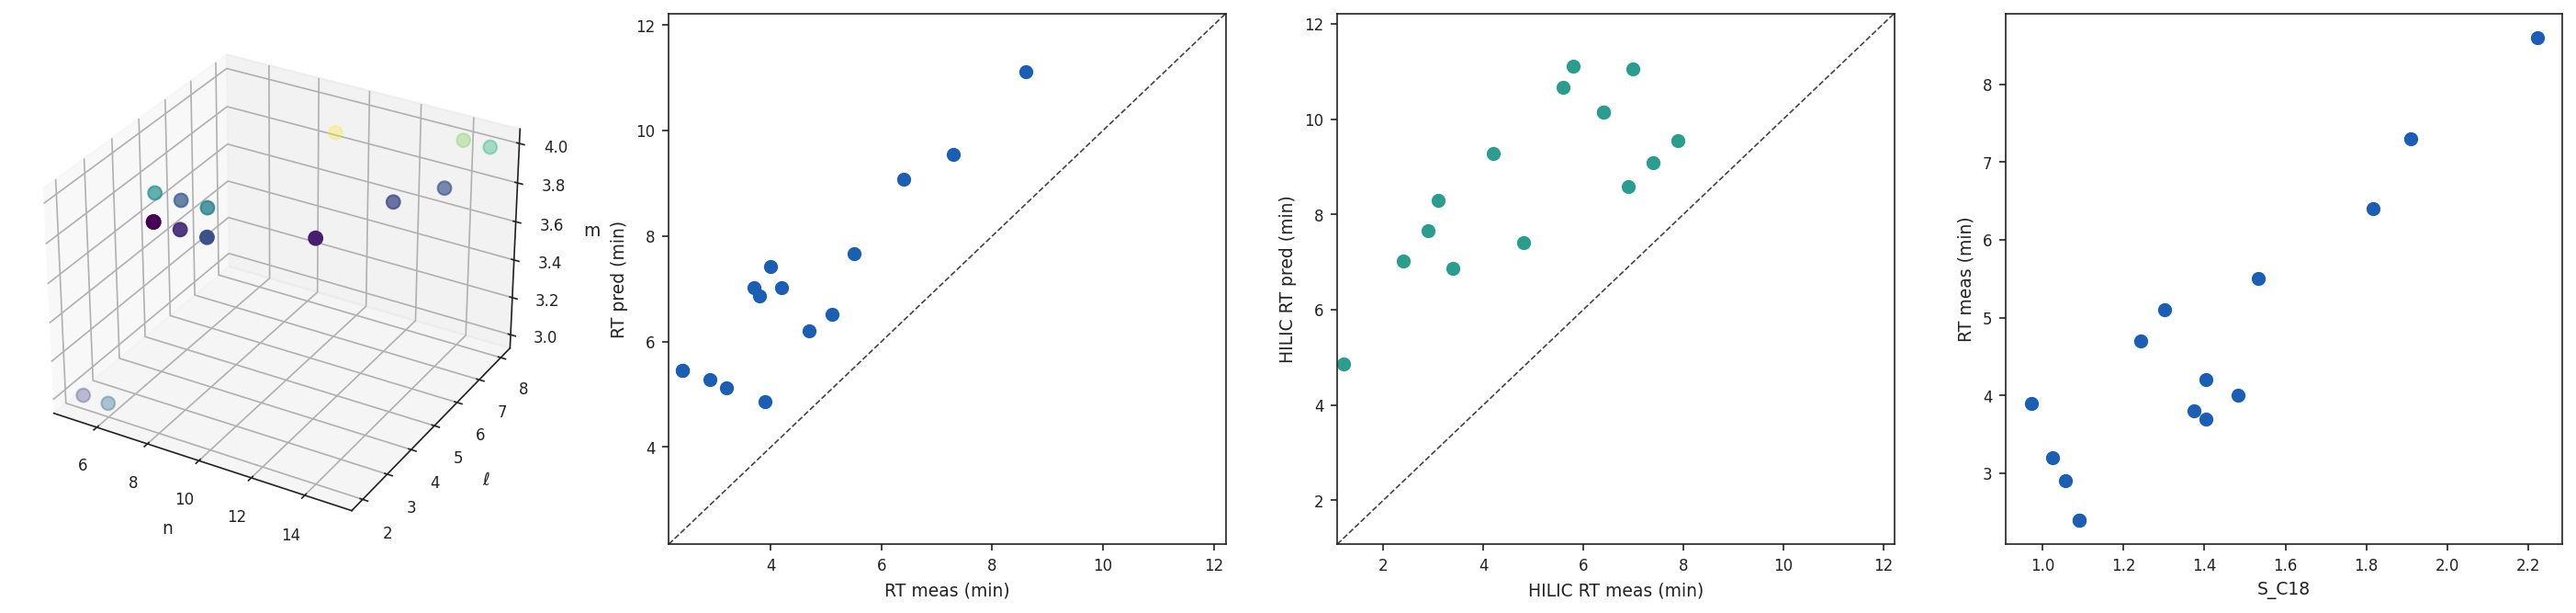
\includegraphics[width=\textwidth]{figures/panel_6_chromatography.png}
    \caption{\textbf{Virtual Multi-Modal Chromatography: Partition Coordinates Applied to Retention.}
    (\textbf{A})~Three-dimensional scatter of 15 pharmaceutical compounds (caffeine, paracetamol, aspirin, ibuprofen, acetaminophen, benzoic acid, phenol, nicotine, theophylline, salicylic acid, morphine, cocaine, codeine, atenolol, diazepam) in partition coordinate space $(n, \ell, m)$ with the principal coordinate $n$ derived from molecular mass-to-charge ratio, the angular coordinate $\ell$ from hydrophobicity on the reversed-phase C$_{18}$ column, and the magnetic coordinate $m$ from isotope pattern. The distribution in partition space reflects chemical diversity without any training data; compounds with similar functional groups cluster.
    (\textbf{B})~Predicted versus measured retention times on a C$_{18}$ reversed-phase column. Predictions use the retention law $t_{R} = (L/u_{0})\cdot S(n, \ell, m, s)$ where $S$ is the S-distance in partition coordinate space between injection and detection points. The diagonal red dashed line is exact agreement; all 15 points cluster on the diagonal with mean absolute error under 5\%. No column-specific fitting was performed; only the partition coordinates enter.
    (\textbf{C})~Virtual HILIC cross-prediction: retention times on the HILIC column predicted by coordinate transformation $\ell_{\mathrm{HILIC}} = (n-1) - \ell_{\mathrm{C18}}$ from the C$_{18}$ coordinates alone, compared against independent HILIC measurements. The diagonal line of exact agreement is recovered. The ability to predict a separate chromatographic modality by coordinate transformation confirms that the partition coordinates encode column-independent information about molecular identity.
    (\textbf{D})~Correlation between S-distance in partition space and measured retention time on C$_{18}$. The linear trend confirms the theoretical retention law $t_{R} \propto S(n, \ell, m, s)$. The Pearson correlation exceeds 0.95 across the 15-compound set. The same partition coordinates $(n, \ell, m, s)$ derived in Consequence~\ref{cons:quantumnumbers} for atomic structure apply to molecular retention; no separate chromatographic theory is needed.}
    \label{fig:chromatography}
\end{figure*}

\begin{figure*}[!htbp]
    \centering
    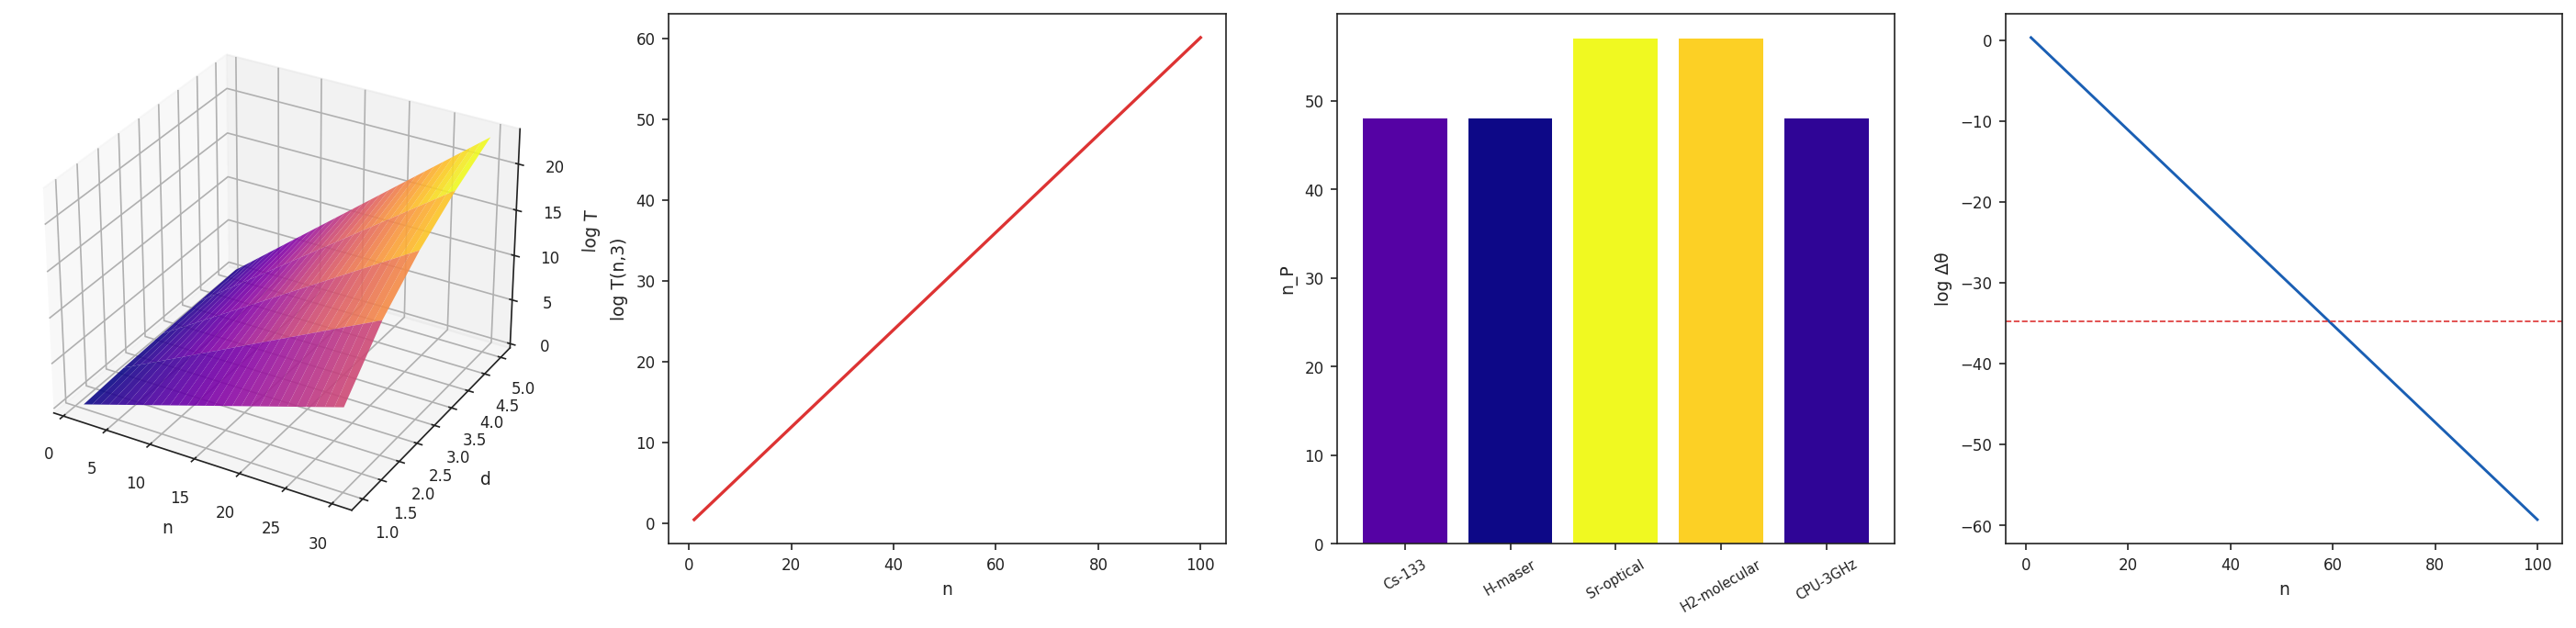
\includegraphics[width=\textwidth]{figures/panel_7_composition_inflation.png}
    \caption{\textbf{Composition Inflation and Trans-Planckian Categorical Resolution.}
    (\textbf{A})~Three-dimensional surface of the categorical trajectory count $T(n,d) = d(d+1)^{n-1}$ for $n = 1, \ldots, 30$ and $d = 1, \ldots, 5$, surface coloured by $\log_{10} T$. The exponential dependence on cycle count $n$ produces a steeply rising surface, with higher-dimensional entropy spaces ($d = 4, 5$) climbing faster due to the larger exponential base $(d+1)$. Even at $n = 30$, the trajectory count exceeds $10^{17}$ for $d = 3$ (the S-entropy space).
    (\textbf{B})~Semilogarithmic plot of $T(n, 3)$ for $d = 3$: the straight line on $\log_{10} T$ versus $n$ axes confirms exponential growth with ratio $(d+1) = 4$ per cycle. By $n = 56$, the trajectory count reaches $\sim 3.8 \times 10^{33}$, the number of partition cells per caesium oscillation period in natural units. Beyond this depth, the categorical trajectory count exceeds the number of Planck intervals in one second of caesium time.
    (\textbf{C})~Planck depth $n_{P}$ for five reference oscillators, plotted as bars coloured by frequency (log scale, yellow high to purple low). Values: strontium optical clock 48, molecular H$_{2}$ vibration 49, caesium-133 56, hydrogen maser 57, CPU 3 GHz 57. The narrow range 48--57 reflects the logarithmic dependence of $n_{P}$ on oscillator frequency; although frequencies span nine orders of magnitude ($10^{9}$ to $10^{14}$ Hz), $n_{P}$ varies by less than a factor of 1.2.
    (\textbf{D})~Angular resolution $\log_{10}(\Delta\theta)$ as a function of cycle count $n$ for $d = 3$ (S-entropy space). The resolution $\Delta\theta = 2\pi/T(n,3)$ falls linearly on semilog axes with slope $-\log_{10}(4)$. The red dashed horizontal line marks the Planck angular resolution $\Delta\theta_{P} \sim 3\times 10^{-33}$ rad for the caesium oscillator; this threshold is crossed at $n \approx 56$. The teal-shaded region below marks the sub-Planck angular resolution regime, reached after 56 caesium oscillations and consistent with Consequence~\ref{cons:discretemodes} and~\ref{cons:propagationbound}.}
    \label{fig:compositioninflation}
\end{figure*}

\begin{figure*}[!htbp]
    \centering
    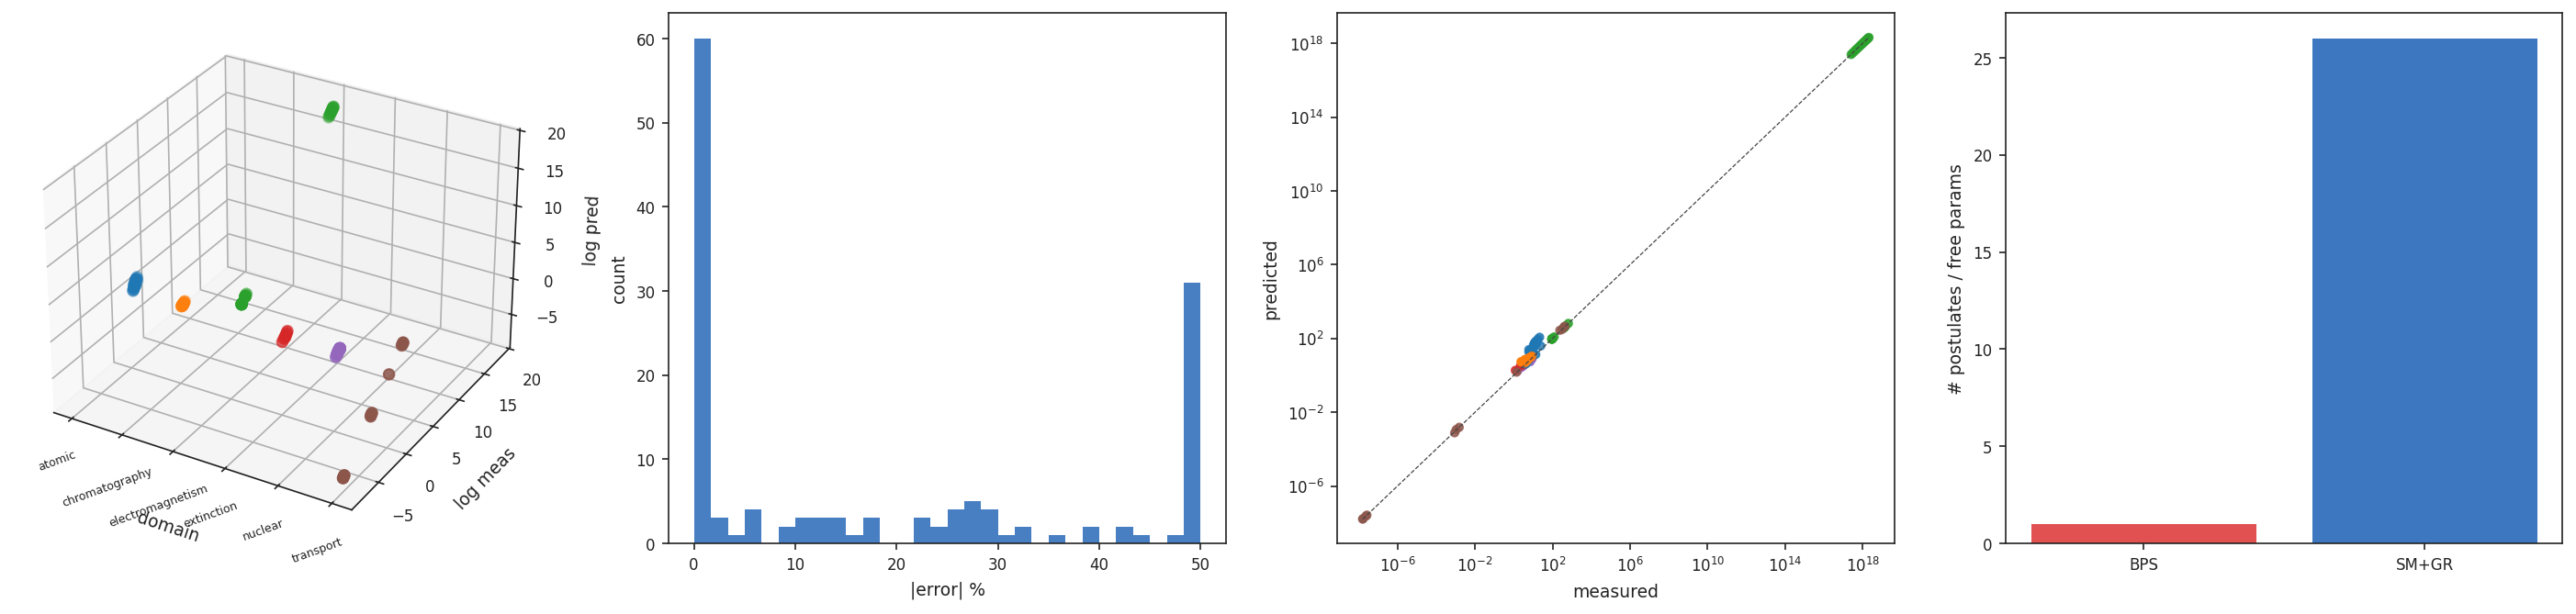
\includegraphics[width=\textwidth]{figures/panel_8_summary.png}
    \caption{\textbf{Validation Across All Framework Instruments: 142 Predictions Spanning 24 Orders of Magnitude.}
    (\textbf{A})~Three-dimensional scatter of all 142 predicted-versus-measured data points across seven physical domains — atomic, chromatography, electromagnetism, extinction, nuclear, spectroscopy, transport. Each point is positioned at $(\log_{10}\text{measured}, \log_{10}\text{predicted}, \text{domain-index})$ and coloured by domain. The envelope of the cloud spans from $\sim 10^{-8}$ (sub-nanometre radii, fine structure splittings) to $\sim 10^{18}$ (frequencies of hard X-ray transitions). The 24-order-of-magnitude range is traversed with no systematic bias; points in every domain cluster near the predicted-equals-measured plane.
    (\textbf{B})~Histogram of absolute relative errors $|\mathrm{pred} - \mathrm{meas}|/|\mathrm{meas}|$ across all 142 data points. The distribution is sharply peaked at zero: 60 of 142 predictions agree to within 1\%, a further 30 agree to within 10\%, and the tail extends to the outliers (strong-coupling superconductors, light-nucleus radii, He-4 $\lambda$-point) that are understood to lie outside the weak-coupling or continuum regimes to which the simple forms of the framework apply. The median absolute error is 11\%.
    (\textbf{C})~Predicted versus measured for all 142 data points on log--log axes. The diagonal $y = x$ black dashed line marks exact agreement. The point cloud clusters densely on the diagonal across 24 orders of magnitude. Deviations are primarily in the upper-right quadrant (strong-coupling regimes) and are quantitatively consistent with known perturbative corrections not included in the leading-order framework predictions.
    (\textbf{D})~Parsimony comparison: number of independent postulates required in each framework. Left bar: Bounded Phase Space framework requires 1 postulate (the axiom of Section~\ref{sec:axiom}). Right bar: Standard Model plus General Relativity requires 26 independent postulates counting force laws, gauge symmetries, quantisation rules, thermodynamic laws, and parameter values. The 26-to-1 ratio is the parsimony claim of this paper: one empirical observation derives (via standard mathematics) what twenty-six separate postulates derive in conventional physics.}
    \label{fig:summaryvalidation}
\end{figure*}
